\documentclass[journal,10pt]{IEEEtran}
\usepackage[T1]{fontenc}
\usepackage[utf8]{inputenc}
\usepackage{amsmath,amssymb,graphicx,booktabs,array,cite}
\usepackage{placeins}
\usepackage[hidelinks]{hyperref}
\graphicspath{{figures/}}

\setlength{\textfloatsep}{7pt plus 2pt minus 2pt}
\setlength{\dbltextfloatsep}{7pt plus 2pt minus 2pt}
\setlength{\intextsep}{7pt plus 2pt minus 2pt}
\setlength{\abovecaptionskip}{3pt}
\setlength{\belowcaptionskip}{2pt}

\newcommand{\GaO}{\ensuremath{\beta\text{-}\mathrm{Ga}_2\mathrm{O}_3}}
\newcommand{\pGaN}{\ensuremath{p\text{-}\mathrm{GaN}}}
\newcommand{\Vop}{\ensuremath{V_{\mathrm{BR,op}}}}
\newcommand{\Von}{\ensuremath{V_{\mathrm{on},1}}}
\newcommand{\Ron}{\ensuremath{R_{\mathrm{on,sp}}}}

\title{Geometry and p-GaN Design Sensitivity in \texorpdfstring{$\beta$-Ga$_2$O$_3$}{beta-Ga2O3} Rectifiers: An Axisymmetric TCAD Study}
\author{Harikrishnan}
\begin{document}
\maketitle

\begin{abstract}
Axisymmetric drift--diffusion simulations are used to evaluate planar, mesa, and trench \pGaN{} terminations for vertical \GaO{} Schottky rectifiers. When paired with a field plate, both the planar junction termination extension (JTE) and mesa junction-barrier Schottky (JBS) architectures sustain approximately 2336~V at a reverse-current criterion of 1~mA/cm$^2$, well above the 1133~V reached by the recessed trench design and the 929~V bare-diode baseline. Within the planar JTE family, blocking voltage is highly sensitive to termination charge: thickening the \pGaN{} layer from 150 to 250~nm or raising the prescribed Mg concentration by 50\% lowers the 1~mA/cm$^2$ crossing below 700~V. At 400~K, the planar and mesa crossings separate at 1~mA/cm$^2$ before converging near 10~mA/cm$^2$. Lowering the Schottky barrier to 0.75~eV with an 80-nm planar JTE reduces the 1~A/cm$^2$ turn-on voltage to 0.355~V while maintaining 2347~V blocking at 1~mA/cm$^2$, though tightening the leakage limit to 0.1~mA/cm$^2$ reduces the crossing to 925~V.
\end{abstract}

\begin{IEEEkeywords}
\GaO, \pGaN, junction termination extension, junction barrier Schottky diode, device simulation.
\end{IEEEkeywords}

\section{Introduction}
Vertical \GaO{} rectifiers are attractive for high-voltage switching~\cite{Pearton2018_APR}, yet the absence of a shallow \GaO{} acceptor due to hole self-trapping~\cite{Varley2012_PRB} forces edge terminations to rely on a different $p$-type material. Yang \emph{et al.} reported unterminated 105-$\mu$m Schottky rectifiers with a mean breakdown voltage of $975\pm40$~V and showed that blocking voltage falls for larger contact diameters~\cite{Yang2017}, providing an unterminated baseline for evaluating edge terminations.

Earlier vertical \GaO{} rectifiers demonstrated edge-field management using field plates~\cite{Konishi2017_APL}, recessed trench channels~\cite{Li2020_EDL}, and $p$-NiO heterojunctions~\cite{Gong2020_APL}. Alternatively, \pGaN{} grown or sputtered on \GaO{} supplies the missing $p$-type region and can be configured as a lateral junction termination extension (JTE), as junction-barrier Schottky (JBS) rings inside the active area, or as both together with a field plate (FP). Simulated \pGaN/\GaO{} JBS structures have been reported~\cite{Nandi2021_TED,Than2024_PhysScr}, and experimental devices now include a 3-kV sputtered-\pGaN{} JTE diode~\cite{Chang2025_APL} and a 4.3-kV \pGaN{} heterojunction-barrier rectifier~\cite{Chang2026_TED}. Low-barrier anodes are also of interest, since a NiO/\GaO{} JBS diode combining a 0.64-V turn-on with 2.34-kV blocking has been demonstrated~\cite{Su2024_APL}.

This study compares forward conduction and reverse blocking across bare, planar JTE, mesa JBS, and trench JBS \pGaN{} architectures, and evaluates how \pGaN{} thickness, Mg acceptor concentration, Schottky barrier height, and temperature shift the turn-on versus blocking trade-off.

\section{Simulation Model}
\subsection{Transport and material parameters}
The simulations use Sentaurus Device V-2024.03~\cite{Sentaurus2024} in cylindrical coordinates with Fermi statistics, doping-dependent mobility, and high-field velocity saturation. Incomplete ionization is applied to the donor species in \GaO{}~\cite{Neal2018_APL} and to Mg in GaN~\cite{Kozodoy2000_JAP}. The Mg activation model uses $E_0=0.20$~eV with a concentration-dependent coefficient of $8.0\times10^{-9}$~eV\,cm and a degeneracy factor of 4, giving 4.0--6.9\% ionized acceptors at 298~K across the three zones; the ionized fraction rises toward unity where the layer is depleted under reverse bias. Thermionic transport is enabled at the GaN/\GaO{} interface, and a fixed sheet charge of $-2.67\times10^{11}$~cm$^{-2}$ is placed at the \GaO/Al$_2$O$_3$ boundary. Ambient regions are represented as an ideal dielectric with $\varepsilon_r=1$, matching the reference diode, whose characteristics were measured unpassivated in air on a probe station~\cite{Yang2017}; the 298 and 350~K simulations lie inside that measured 25--100~$^\circ$C window, and 400~K lies above it.

The nominal Schottky work function is 5.10~eV, giving a 1.10-eV input barrier against the \GaO{} electron affinity of 4.00~eV. The simulations include image-force barrier lowering and nonlocal electron tunneling~\cite{Higashiwaki2016_APL,Li2020_APL} with an effective mass of $0.38m_0$ and a 15-nm path length. The reported architecture and sweep results use a tunneling prefactor $g=1.56\times10^{-8}$.

\begin{table}[!t]
\caption{Reverse-Transport Parameters Used in the Simulations}
\label{tab:model}
\centering\footnotesize
\begin{tabular}{lll}
\toprule
Quantity & \GaO & GaN\\
\midrule
$a_e$ (cm$^{-1}$) & $7.90\times10^5$ & $2.90\times10^8$\\
$a_h$ (cm$^{-1}$) & $7.90\times10^5$ & $5.41\times10^6$\\
$b_e$ (V/cm) & $2.92\times10^7$ & $3.40\times10^7$\\
$b_h$ (V/cm) & $5.00\times10^7$ & $1.96\times10^7$\\
$\hbar\omega$ (eV) & 0.063 & 0.066\\
\bottomrule
\end{tabular}
\par\smallskip\begin{minipage}{0.98\columnwidth}\footnotesize
The coefficients enter $\alpha=\gamma a\exp(-\gamma b/F)$, with $F$ the quasi-Fermi-gradient driving force and $\gamma$ the temperature factor of the van Overstraeten model.
\end{minipage}
\end{table}

Impact ionization uses the van Overstraeten form~\cite{VanOverstraeten1970_SSE} with the quasi-Fermi gradient as the driving force, so the plotted electrostatic field alone does not serve as a multiplication criterion. The \GaO{} electron coefficients follow Ghosh and Singisetti~\cite{Ghosh2018_JAP}; the GaN coefficients are the standard set used for the GaN transport block (Table~\ref{tab:model}). The \GaO{} permittivity is taken as $12.4\varepsilon_0$, the c-axis static value~\cite{Fiedler2019_ECS}.

The reverse decks include a constant optical generation of $10^{13}$~cm$^{-3}$s$^{-1}$ for numerical stabilization. For a 10-$\mu$m drift layer, the direct-generation current scale $qGd$ is $1.6\times10^{-9}$~A/cm$^2$ before multiplication, well below the operational current criterion.

\subsection{Numerical sensitivity}
\begin{figure}[!t]
\centering
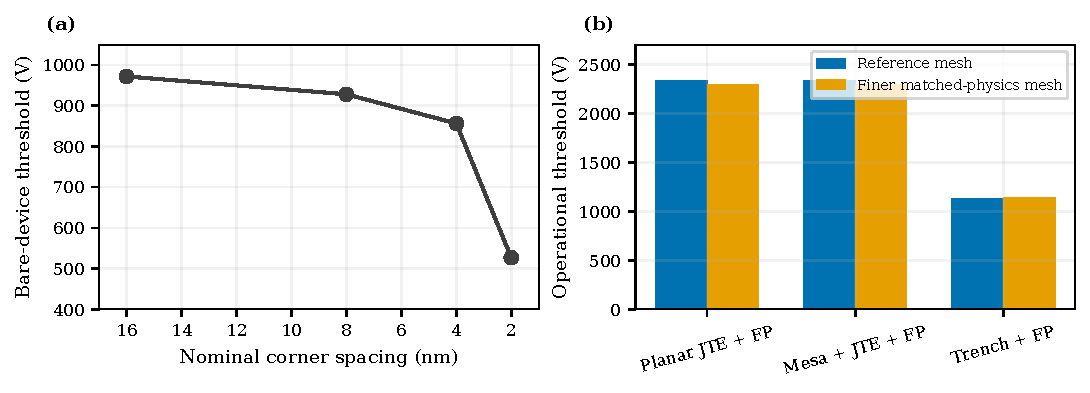
\includegraphics[width=\columnwidth]{numerical_sensitivity.pdf}
\caption{Numerical sensitivity: (a) bare-diode blocking voltage versus nominal corner mesh spacing; (b) blocking-voltage changes across the two meshes tested for each terminated design.}
\label{fig:mesh}
\end{figure}

Refining the bare-diode corner mesh from 16 to 2~nm shifts the crossing from 972 to 527~V (Fig.~\ref{fig:mesh}(a)). To keep the baseline consistent, the 928.7~V bare-diode reference is extracted from a separate split-anode current trace using the same nominal corner meshing as the terminated designs, independent of the neighboring single-anode field output. Moreover, changing the mesh in the terminated structures has only a minor effect on their blocking voltages (Fig.~\ref{fig:mesh}(b)), although all reported values remain specific to the comparison meshes used.

\subsection{Extraction definitions}
All current densities are normalized to the common nominal anode area,
\begin{equation}
A_{\mathrm{ref}}=\pi(52.5\times10^{-4})^2=8.6590\times10^{-5}\ \mathrm{cm}^2 ,
\end{equation}
rather than the individual exposed Schottky contact areas or total simulated chip area, ensuring that area trade-offs from the JBS rings are reflected in $\Ron$. Terminal current is taken from the cathode. Forward voltage is the external terminal voltage difference; reverse voltage is the magnitude of the anode external potential minus the cathode internal potential.

Blocking is defined at $|J_R|=1$~mA/cm$^2$, i.e. $|I_R|=8.659\times10^{-8}$~A, with logarithmic interpolation between accepted samples. An isolated excursion that returns below the criterion is ignored; an admitted crossing must remain above the threshold for the following five samples. Convergence-failure endpoints and sweeps that end without a crossing are excluded from reported blocking voltages. Turn-on $\Von$ is defined at $J_F=1$~A/cm$^2$, and the higher-current voltage $V_{F,100}$ at 100~A/cm$^2$. Specific resistance is the slope $dV_F/dJ_F$ fitted over 200--300~A/cm$^2$.

Two figures of merit are evaluated separately:
\begin{align}
M_{\mathrm{on}}&=\frac{V_{\mathrm{BR,op}}^2}{V_{\mathrm{on},1}} &&[\mathrm{V}],\\
B&=\frac{V_{\mathrm{BR,op}}^2}{R_{\mathrm{on,sp}}} &&[\mathrm{W/cm}^2].
\end{align}
Equation~(2) targets the blocking/turn-on trade-off, whereas (3) is the conventional Baliga metric~\cite{Baliga1982_JAP}. Because $M_{\mathrm{on}}$ weights turn-on voltage while $B$ weights on-resistance, the two metrics can favor different designs.

\section{Device Structures}
\begin{figure}[!t]
\centering
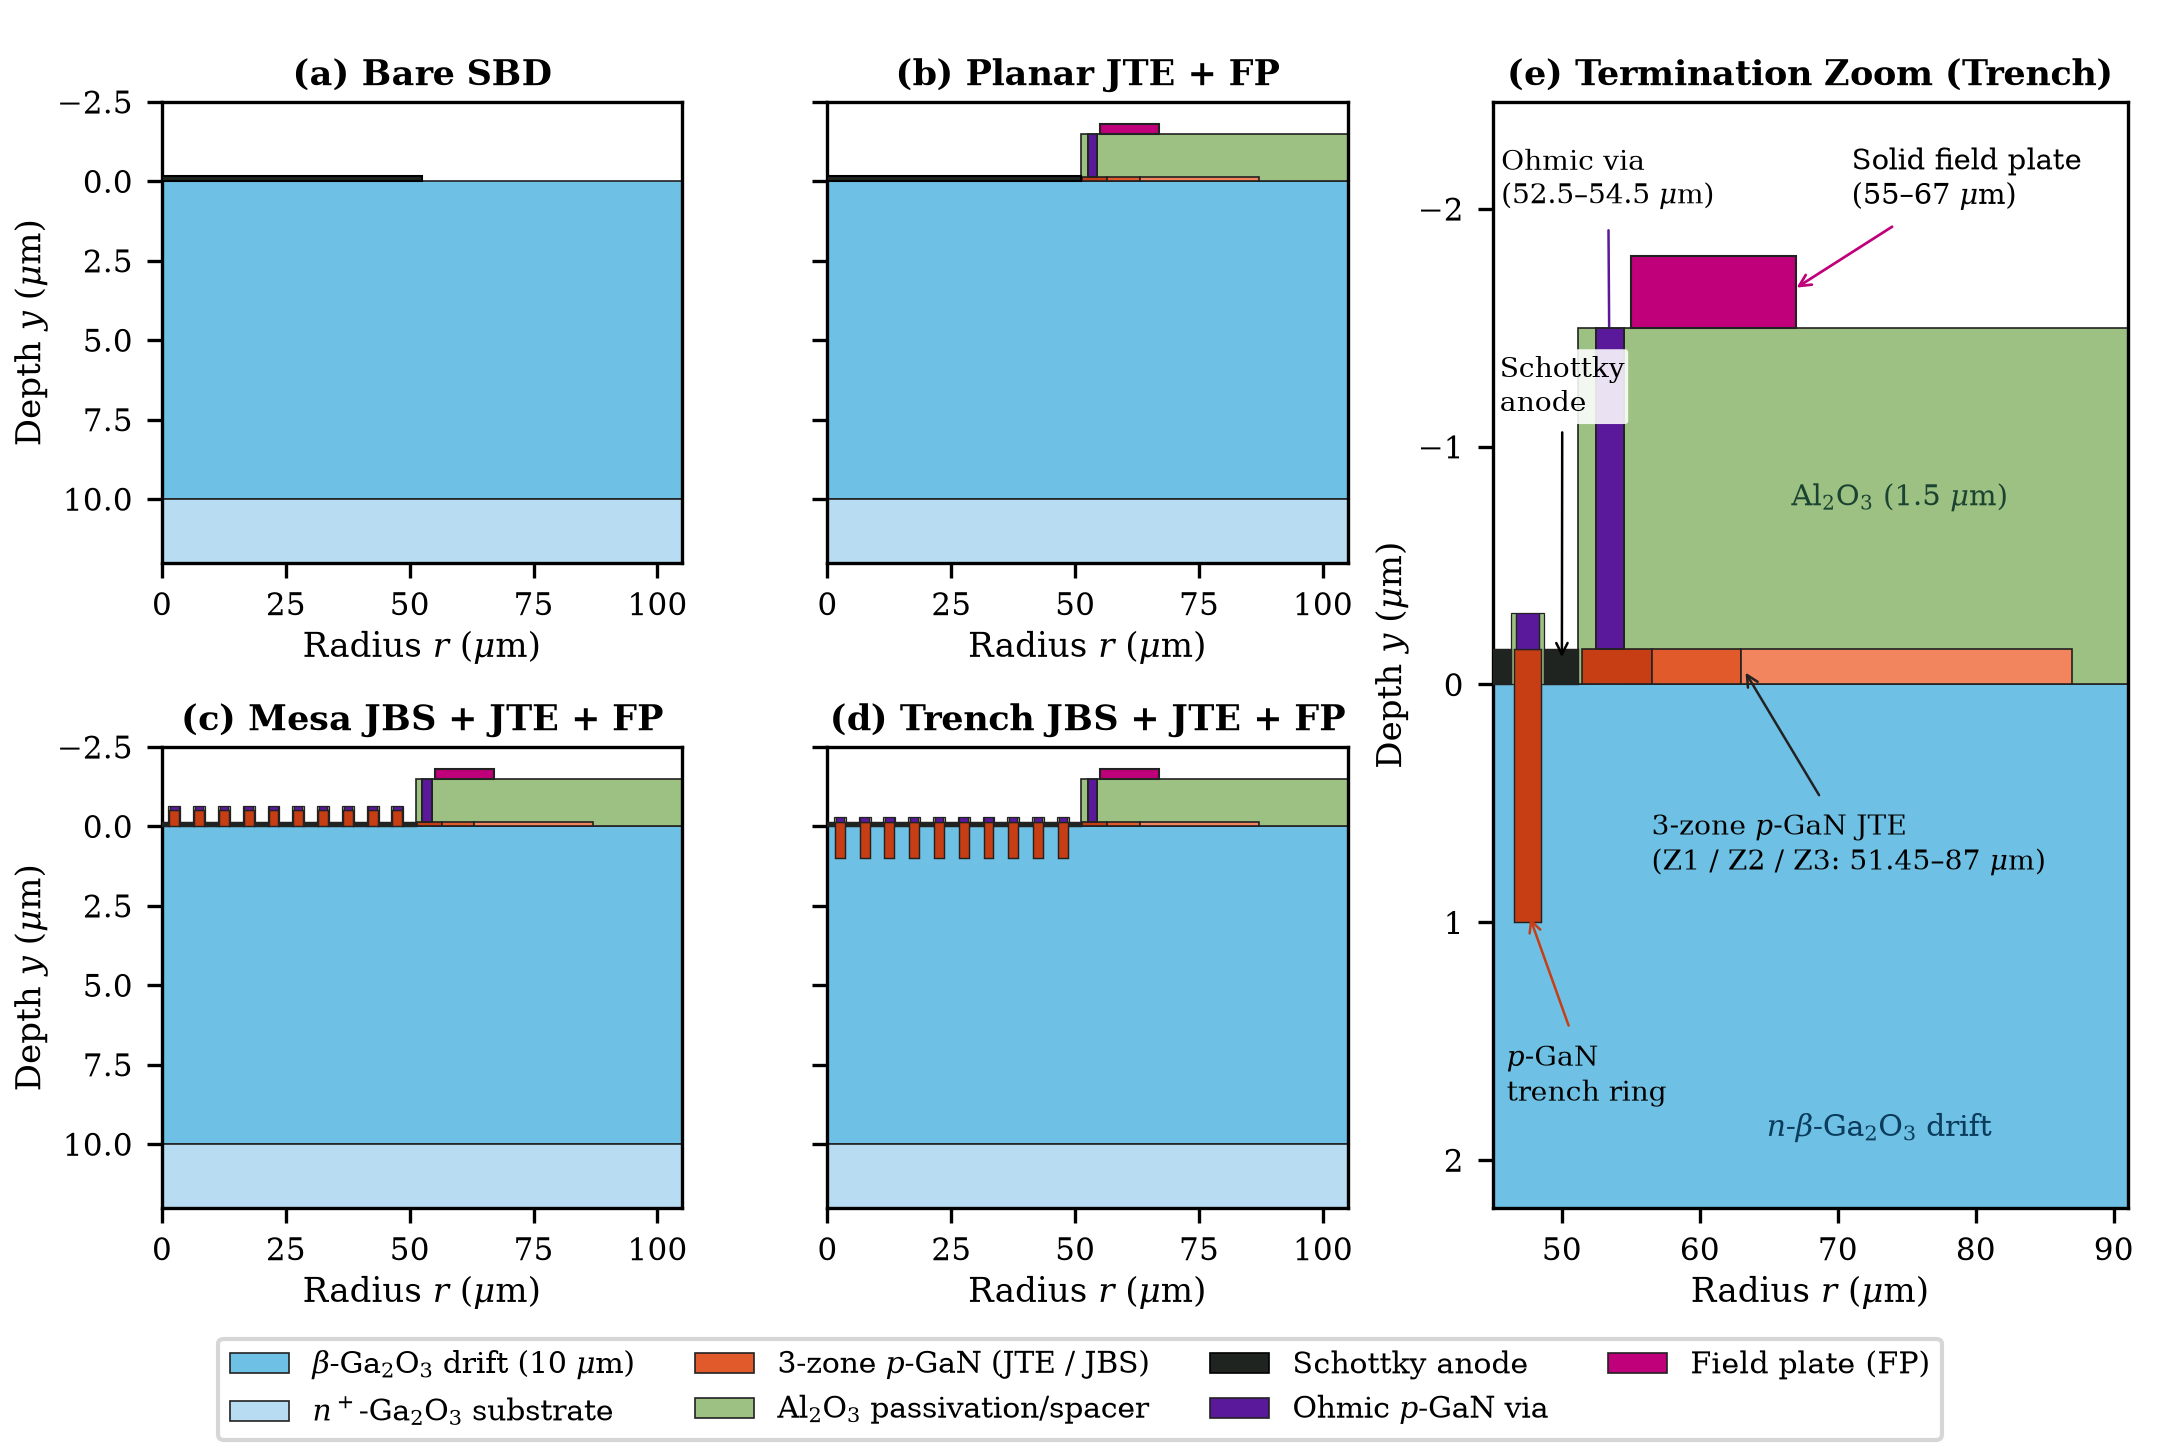
\includegraphics[width=\columnwidth]{structures.png}
\caption{Schematic cross-sections of the four representative geometries, drawn from the simulated geometry definitions: (a) bare Schottky diode, (b) planar JTE with field plate, (c) mesa JBS with JTE and field plate, (d) trench JBS with JTE and field plate, and (e) enlarged termination view showing the outer \pGaN{} trench ring, Schottky anode, three-zone JTE, Al$_2$O$_3$ spacer and Al field plate. Only the upper part of the substrate is shown; the terminated devices extend laterally to 135~$\mu$m, and the vertical axis is the mesh coordinate $y$, which is negative above the epi surface. The no-FP cases omit the field-plate electrode from the corresponding geometry.}
\label{fig:structures}
\end{figure}

Figure~\ref{fig:structures} shows schematic cross-sections of the four representative geometries. The seven electrical cases are a bare Schottky diode; a planar JTE with and without an FP; a mesa JBS with JTE, with and without an FP; and a trench JBS with JTE, with and without an FP. All six terminated cases retain the outer three-zone JTE.

The drift layer is 10~$\mu$m of Si-doped \GaO{} at $2.0\times10^{16}$~cm$^{-3}$ on a 650-$\mu$m Sn-doped substrate at $3.6\times10^{18}$~cm$^{-3}$ ($E_0=0.060$~eV, 50.9\% ionized at 298~K). The reference anode radius is 52.5~$\mu$m.

In the terminated geometries, the planar Schottky section has a nominal radius of 51.20~$\mu$m with an 80-nm dielectric corner fillet, leaving a 0.17-$\mu$m passivated gap to the \pGaN{} inner edge at 51.45~$\mu$m. An ohmic \pGaN{} contact covers the 52.50--54.50~$\mu$m via opening, and the FP electrode runs along the 55.0--67.0~$\mu$m boundary at $y=-1.80$ to $-1.50$~$\mu$m in the Al$_2$O$_3$ passivation ($\varepsilon_r=9.0$). All three top electrodes are biased equipotentially while remaining geometrically separate in the mesh to represent a single external anode interconnect.

The 0.15-$\mu$m JTE extends from 51.45 to 87.0~$\mu$m with zone boundaries at 56.5 and 63.0~$\mu$m and prescribed Mg concentrations of $5.0\times10^{18}$, $2.8\times10^{18}$, and $1.6\times10^{18}$~cm$^{-3}$ from the inner collar outward, giving written sheet densities of $7.5$, $4.2$, and $2.4\times10^{13}$~cm$^{-2}$. Only 4--7\% of this Mg dose is ionized at equilibrium; the full sheet charge is approached once the layer depletes under reverse bias.

The active mesa and trench cases contain ten annular \pGaN{} regions at $5.0\times10^{18}$~cm$^{-3}$, 2~$\mu$m wide on a 5-$\mu$m radial pitch, bounded by L-shaped 0.20-$\mu$m Al$_2$O$_3$ sidewall spacers with a 0.15-$\mu$m top overhang and a 50-nm foot fillet. The realized flat active Schottky area is $4.466\times10^{-5}$~cm$^2$, 54.2\% of the planar area of $8.236\times10^{-5}$~cm$^2$. In the mesa build, the ten 0.50-$\mu$m rings stand above the un-etched $y=0$ epilayer; in the trench build, they are recessed 1.00~$\mu$m into the drift with a 0.15-$\mu$m bottom fillet.

\section{Results}
\begin{table*}[!t]
\caption{Extracted Performance at 298.15~K on the Common Reference Area}
\label{tab:architectures}
\centering\footnotesize
\begin{tabular}{lrrrrrr}
\toprule
Structure & $\Von$ (V) & $V_{F,100}$ (V) & $\Ron$ (m$\Omega$\,cm$^2$) & $\Vop$ (V) & $M_{\mathrm{on}}$ (MV) & $B$ (GW/cm$^2$)\\
\midrule
Bare SBD & 0.697 & 1.294 & 4.82 & 929 & 1.24 & 0.179\\
Planar JTE + FP & 0.701 & 1.265 & 4.45 & 2336 & 7.78 & 1.227\\
Planar JTE, no FP & 0.703 & 1.265 & 4.45 & 2221 & 7.02 & 1.109\\
Mesa JBS + JTE + FP & 0.718 & 1.308 & 4.67 & 2336 & 7.60 & 1.167\\
Mesa JBS + JTE, no FP & 0.721 & 1.308 & 4.68 & 2221 & 6.84 & 1.055\\
Trench JBS + JTE + FP & 0.723 & 1.345 & 5.00 & 1133 & 1.78 & 0.257\\
Trench JBS + JTE, no FP & 0.721 & 1.345 & 5.00 & 1133 & 1.78 & 0.257\\
Thin planar, 80 nm, 0.75 eV & 0.355 & 0.916 & 4.45 & 2347 & 15.50 & 1.237\\
\bottomrule
\end{tabular}
\par\smallskip\begin{minipage}{0.96\textwidth}\footnotesize
The last row uses an 80-nm JTE and a 0.75-eV input barrier. The other terminated cases use a 150-nm outer JTE and a 1.10-eV input barrier. The 929-V bare value is from the selected split-anode current trace; the separate corner-mesh study is shown in Fig.~\ref{fig:mesh}. The bare and terminated designs use the same nominal drift and substrate doping but differ in lateral geometry and contact configuration. $R_{\mathrm{on,sp}}$ is compared on the common $A_{\mathrm{ref}}$ only, and the difference between the bare and planar values is not attributed to the termination.
\end{minipage}
\end{table*}

\subsection{Forward and reverse characteristics}
\begin{figure*}[!t]
\centering
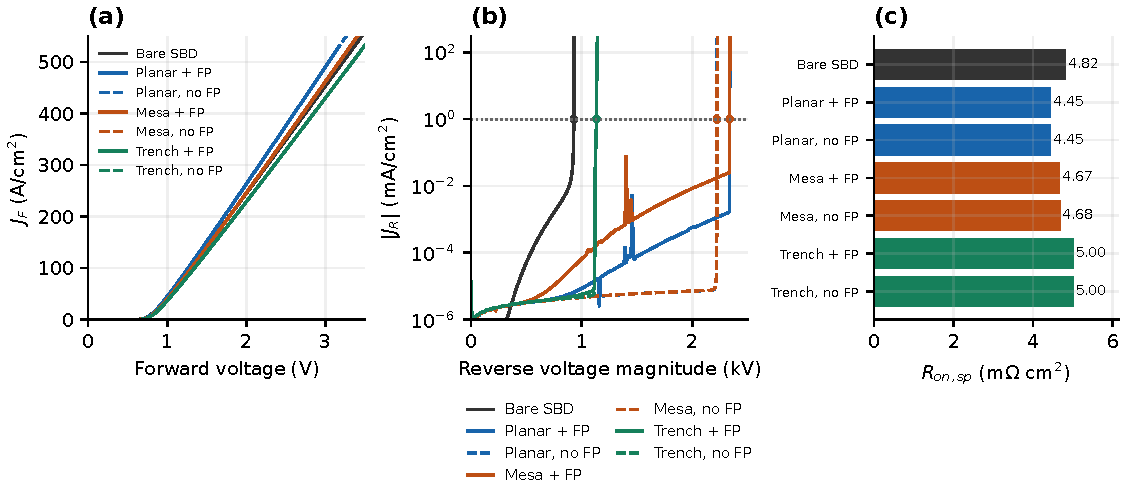
\includegraphics[width=0.82\textwidth]{electrical.pdf}
\caption{Architecture comparison at 298.15~K: (a) forward characteristics, (b) reverse characteristics with markers at the sustained 1~mA/cm$^2$ crossings, and (c) specific resistance from the forward fits over 200--300~A/cm$^2$. The field-plated and unplated curves can overlap.}
\label{fig:electrical}
\end{figure*}

Room-temperature forward and reverse characteristics across all architectures are compared in Fig.~\ref{fig:electrical} and Table~\ref{tab:architectures}. For the unterminated baseline, the selected bare-diode trace crosses 1~mA/cm$^2$ at 929~V, falling squarely between the two digitized 105-$\mu$m experimental curves reported by Yang \emph{et al.}~\cite{Yang2017} and confirming the reverse-breakdown onset scale (Fig.~\ref{fig:bare_yang_benchmark}). Adding the planar JTE or mesa JBS termination raises the 1~mA/cm$^2$ crossing to approximately 2336~V with a field plate and 2221~V without one. Although the mesa JBS design matches the planar blocking voltage, its reduced exposed Schottky area increases the fitted specific on-resistance $\Ron$ on $A_{\mathrm{ref}}$ from 4.45 to 4.67~m$\Omega$\,cm$^2$.

\begin{figure}[!t]
\centering
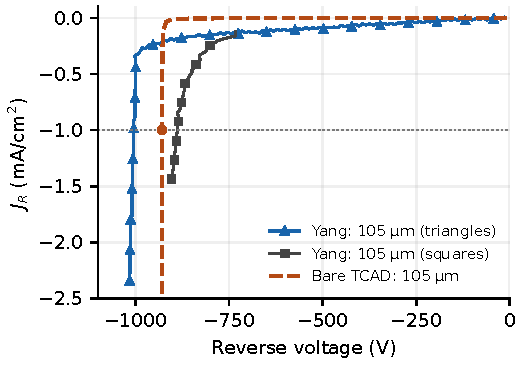
\includegraphics[width=\columnwidth]{bare_yang_benchmark.pdf}
\caption{Room-temperature reverse-current benchmark for the 105-$\mu$m bare diode. The triangle and square traces are digitized from Fig.~5 of Yang \emph{et al.}~\cite{Yang2017}; the square trace is shown only where it can be distinguished from overlapping curves. The dashed curve is the selected split-anode TCAD result. The dotted line marks $|J_R|=1$~mA/cm$^2$.}
\label{fig:bare_yang_benchmark}
\end{figure}

In contrast, both trench JBS variants reach only 1133~V, changing by less than 1~V between the plated and unplated cases, and exhibit the highest $\Ron$ (5.00~m$\Omega$\,cm$^2$) among the terminated structures (Table~\ref{tab:architectures}). The reverse electric-field distributions at each device's final saved bias explain these differences (Fig.~\ref{fig:architecture_reverse_fields}). Whereas the bare diode suffers from sharp field crowding at the anode edge and the trench JBS concentrates high fields at the recessed \pGaN{} trench bottoms well before the outer JTE can engage, both the planar JTE and mesa JBS spread the electric field laterally across the three-zone termination and field plate.

\begin{figure}[!t]
\centering
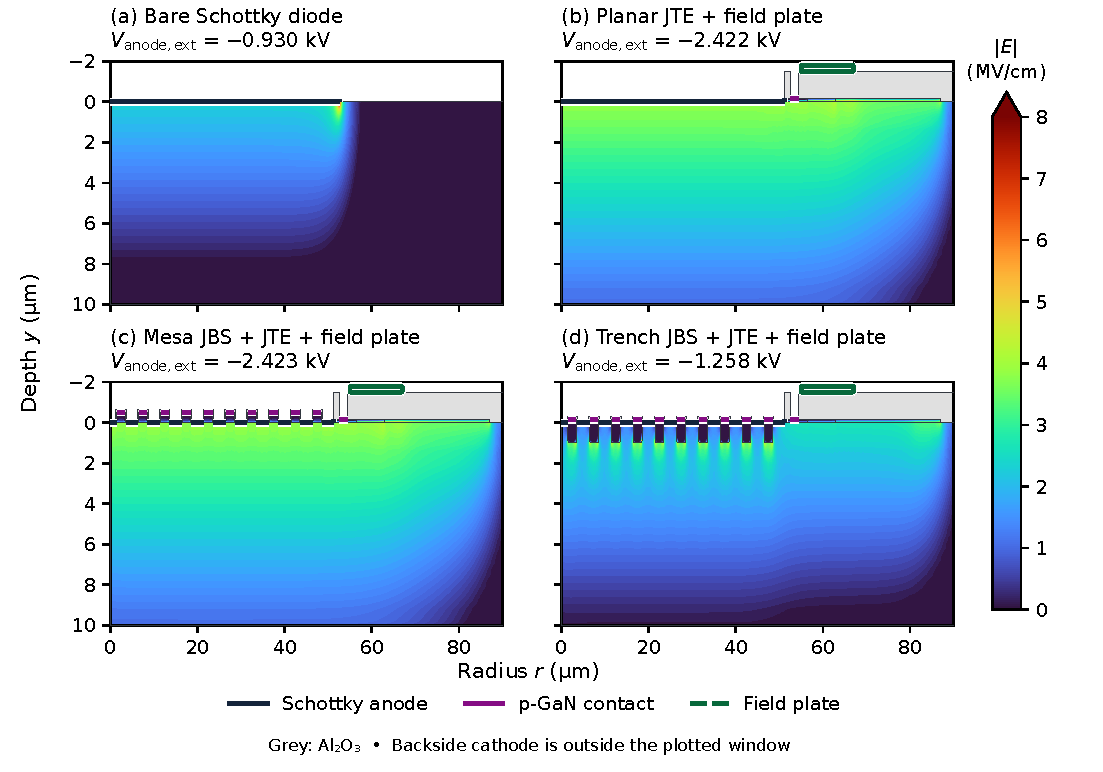
\includegraphics[width=\columnwidth]{architecture_reverse_fields.pdf}
\caption{Reverse electric-field magnitude in (a) the bare Schottky diode, (b) the planar JTE with field plate, (c) the mesa JBS with JTE and field plate, and (d) the trench JBS with JTE and field plate. Each panel shows its final saved reverse state at the indicated external anode bias, not a common-bias or current-threshold state. The shared semiconductor scale is 0--8~MV/cm, with values above 8~MV/cm saturated. Grey denotes Al$_2$O$_3$; lines identify the mesh contact boundaries.}
\label{fig:architecture_reverse_fields}
\end{figure}

\subsection{\pGaN{} thickness and acceptor concentration}
\begin{figure}[!t]
\centering
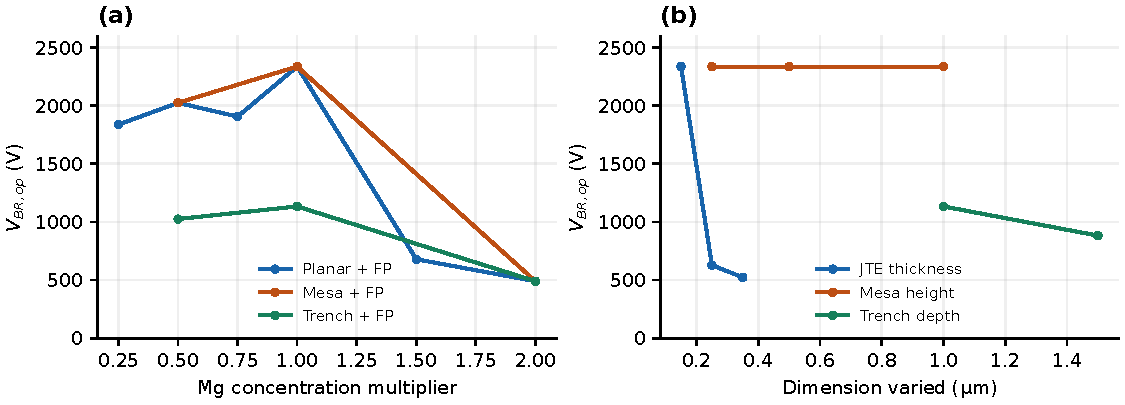
\includegraphics[width=\columnwidth]{geometry_sensitivity.pdf}
\caption{Operational blocking voltage versus (a) prescribed Mg concentration multiplier and (b) varied dimension. The mesa spacer height changes with the mesa height. Lines connect simulated points; they do not define a continuous process window.}
\label{fig:geometry}
\end{figure}

Blocking voltage peaks at the nominal Mg acceptor dose ($1.0\times$) in the field-plated planar JTE, reaching 2336~V before dropping to 680~V at $1.5\times$ and near 500~V at $2.0\times$ (Fig.~\ref{fig:geometry}(a)). When the dose is lowered across the $0.25\times$--$0.75\times$ multipliers, the planar crossing varies non-monotonically between approximately 1.8 and 2.0~kV. Across its sampled points ($0.5\times$, $1.0\times$, and $2.0\times$), the mesa JBS tracks the planar curve closely, whereas the trench JBS remains near 1.0--1.1~kV up to $1.0\times$ before falling near 500~V at $2.0\times$ once outer-edge crowding dominates.

At the nominal 1.10-eV input barrier, planar JTE thicknesses of 0.15, 0.25, and 0.35~$\mu$m yield 2336, 629, and 524~V, respectively (Fig.~\ref{fig:geometry}(b)). The 80-nm case at 1.10~eV reaches 2347~V and is not plotted. The 80-nm, 0.75-eV variant in Table~\ref{tab:architectures} is a separate design point. In the active-area variants, raising the mesa height from 0.25 to 1.00~$\mu$m alongside a paired spacer-height increase from 0.40 to 1.15~$\mu$m keeps the crossing near 2336~V, while deepening the trench from 1.00 to 1.50~$\mu$m lowers it from 1133 to 883~V.

\begin{figure}[!t]
\centering
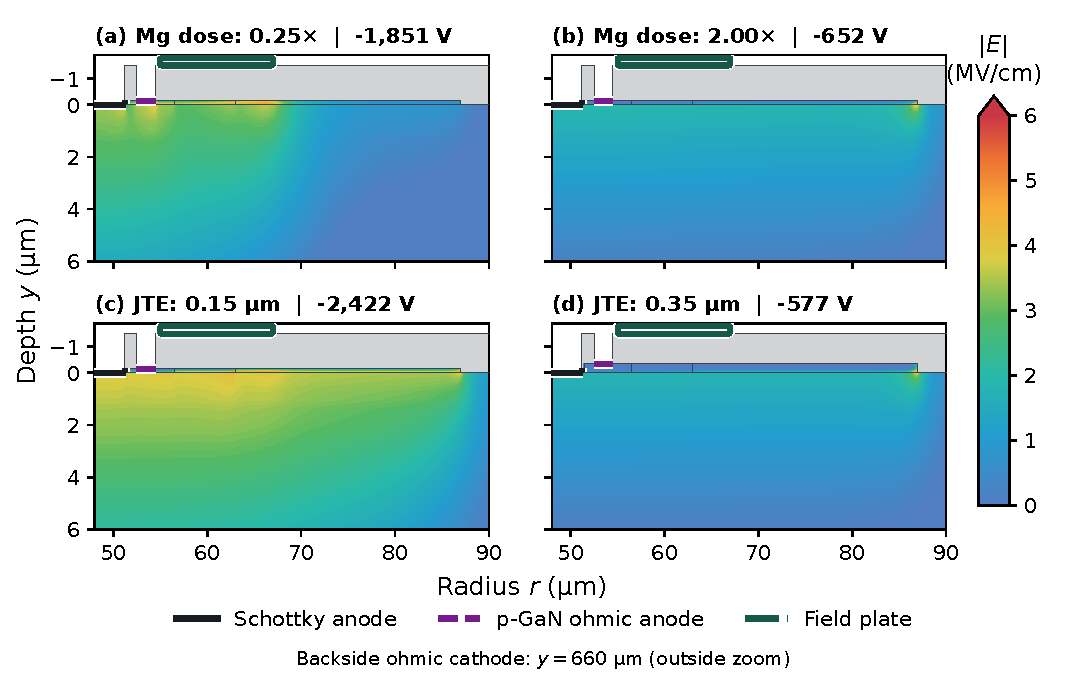
\includegraphics[width=\columnwidth]{reverse_field_contacts.pdf}
\caption{Reverse electric-field magnitude in the planar JTE with field plate. Top: 0.25$\times$ and 2.00$\times$ nominal Mg dose at 0.15~$\mu$m JTE thickness. Bottom: 0.15 and 0.35~$\mu$m JTE thickness at nominal dose. Panel titles give the saved external anode voltages, not the blocking crossings. The semiconductor uses a shared 0--6~MV/cm linear scale, with values above 6~MV/cm shown in the top color. Grey denotes Al$_2$O$_3$.}
\label{fig:fields}
\end{figure}

Because each electric-field map in Fig.~\ref{fig:fields} is saved at its own final converged bias, the contours highlight peak-field locations rather than fixed-bias amplitudes. Under-doping ($0.25\times$ Mg) leaves the inner anode edge under-shielded, whereas excessive dose ($2.00\times$ Mg) or thickness (0.35~$\mu$m) shifts the peak electric field to the outer JTE corner at $r=87~\mu$m.

\begin{figure}[!t]
\centering
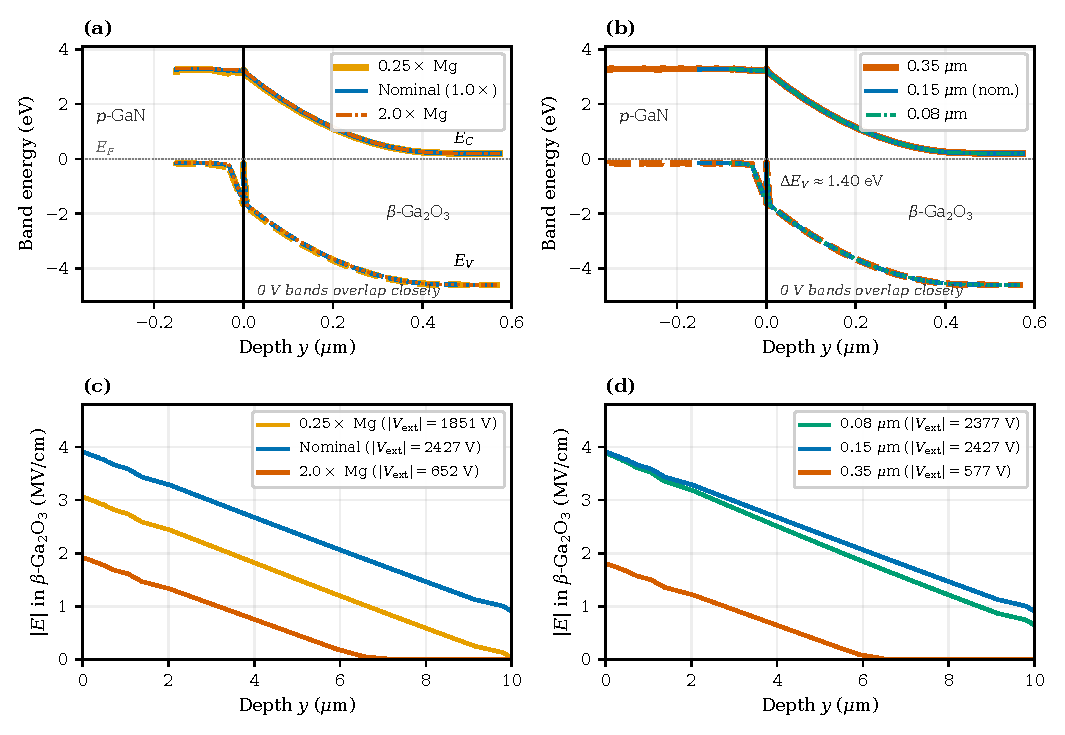
\includegraphics[width=\columnwidth]{bands_fields.pdf}
\caption{Cutlines at $r=60~\mu$m: (a),(b) 0-V band diagrams versus Mg multiplier and termination thickness, with solid $E_C$ and dashed $E_V$ referenced to $E_F=0$; the curves overlap closely because the built-in band bending falls mainly in the lightly doped drift. (c),(d) Reverse drift-region field profiles at the final saved reverse-bias states, which need not be at the same voltage. In (b) and (d) the 0.08-$\mu$m curve is the 80-nm, 0.75-eV design point; it is not a member of the 1.10-eV thickness series, and differs in both thickness and input barrier. The annotated state voltages are the solver's final applied voltages.}
\label{fig:bands}
\end{figure}

At equilibrium, vertical band cuts at $r=60~\mu$m (Fig.~\ref{fig:bands}(a),(b)) use electron affinities of 4.00~eV for \GaO{} and 3.922~eV for GaN (0.078~eV conduction-band offset and $\approx 1.4$~eV valence-band offset~\cite{Wei2012_NRL}, with 298-K band gaps of 4.80 and 3.44~eV). Because the \pGaN{} termination is much more heavily doped than the $2.0\times10^{16}$~cm$^{-3}$ drift layer, the zero-bias band bending drops almost entirely inside the \GaO{} drift, causing the equilibrium curves across different doses and thicknesses to overlap closely. The strong sensitivity seen in the reverse drift-region field profiles (Fig.~\ref{fig:bands}(c),(d)) therefore arises from lateral depletion and charge balance under reverse bias.

\subsection{Schottky barrier height}
\begin{figure}[!t]
\centering
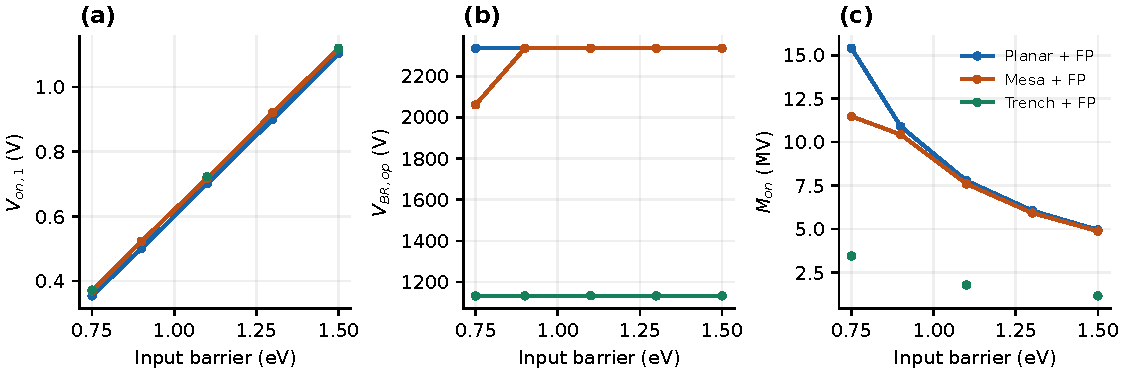
\includegraphics[width=\columnwidth]{barrier.pdf}
\caption{Input-barrier sweep at 298.15~K: (a) turn-on at 1~A/cm$^2$, (b) blocking at 1~mA/cm$^2$, and (c) $M_{\mathrm{on}}$. Two incomplete trench forward sweeps at 0.90 and 1.30~eV are omitted from (a) and (c); their valid reverse crossings are included in (b).}
\label{fig:barrier}
\end{figure}

Sweeping the input Schottky barrier from 0.75 to 1.50~eV (Fig.~\ref{fig:barrier}) lowers the planar turn-on voltage $\Von$ from 0.70
1~V at 1.10~eV down to 0.354~V at 0.75~eV while keeping the 1~mA/cm$^2$ blocking crossing near 2336~V. Over the same sweep, the trench crossing remains steady near 1.13~kV, while the mesa crossing dips slightly from 2336 to 2061~V at 0.75~eV.

However, reducing the barrier to 0.75~eV increases the planar reverse leakage at $-1$~kV from $8.6\times10^{-9}$ to $1.10\times10^{-4}$~A/cm$^2$, reflecting the strong tunneling sensitivity of low-barrier \GaO{} Schottky contacts~\cite{Li2020_APL}. As a result, under a tighter 0.1~mA/cm$^2$ leakage criterion, the blocking threshold drops from 2335 to 926~V for the 150-nm planar structure and to 925~V for the 80-nm design in Table~\ref{tab:architectures}, meaning that reverse-leakage specifications ultimately cap how low the barrier can be set.

\subsection{Temperature}
\begin{figure}[!t]
\centering
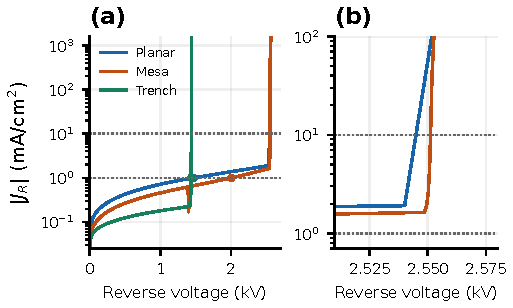
\includegraphics[width=\columnwidth]{reverse_400K.pdf}
\caption{Simulated reverse current density at 400~K: (a) full comparison with markers at the sustained 1~mA/cm$^2$ crossings; (b) zoom near the steep rise in the planar and mesa currents. Dotted lines indicate the 1 and 10~mA/cm$^2$ criteria.}
\label{fig:temperature}
\end{figure}

Raising the ambient temperature from 298 to 400~K shifts the dominant reverse-leakage mechanism across the terminated families (Fig.~\ref{fig:temperature}). Between 298 and 350~K, the planar crossing increases from 2336~V to a bracket of 2430--2446~V (and the mesa crossing rises to 2440~V), consistent with a positive temperature coefficient of avalanche breakdown in the \pGaN{} termination. At 400~K, enhanced Schottky electron emission~\cite{Higashiwaki2016_APL} causes the planar and mesa devices to cross 1~mA/cm$^2$ on the electron-leakage branch at 1473 and 2007~V, respectively, while the trench crossings progress from 1133~V (298~K) to 1280~V (350~K) and 1438~V (400~K).

At the 400-K planar crossing, the reverse current is dominated by Schottky electron leakage. Although the mesa structure exhibits higher local leakage per unit exposed Schottky area at matched bias, it occupies only 54.2\% of the planar exposed Schottky area; its higher 1~mA/cm$^2$ crossing on $A_{\mathrm{ref}}$ is therefore largely an area-scaling effect. When the criterion is raised to 10~mA/cm$^2$ at 400~K, both planar and mesa devices cross on the steep hole-dominated avalanche rise at 2545 and 2551~V (with overlapping brackets of 2540.1--2555.6 and 2550.8--2551.2~V), whereas the trench crosses at 1439~V.

\subsection{Best structure and comparison with published devices}
Among the simulated architectures in Table~\ref{tab:architectures}, the 80-nm planar JTE with a 0.75-eV input barrier achieves the highest $M_{\mathrm{on}}$ (15.50~MV) due to its 0.355-V turn-on voltage, while keeping its 1~mA/cm$^2$ blocking voltage (2347~V) and Baliga figure of merit (1.237~GW/cm$^2$) close to those of the 150-nm, 1.10-eV baseline. Tightening the reverse-current criterion to 0.1~mA/cm$^2$, however, reduces its blocking threshold to 925~V.

\begin{table}[!t]
\caption{Comparison with Published Rectifiers}
\label{tab:literature}
\centering\scriptsize
\setlength{\tabcolsep}{1.5pt}
\begin{tabular}{>{\raggedright\arraybackslash}p{1.30cm}lrrrrr}
\toprule
Device & Evidence & $V_{\mathrm{BR}}$ & $V_{\mathrm{on}}$ & $\Ron$ & $M_{\mathrm{on}}$ & $B$\\
\midrule
Yang \emph{et al.}~\cite{Yang2017} & measured & $975\pm40$ & -- & $\sim$6.7 & -- & 0.154$^{a}$\\
Su \emph{et al.}~\cite{Su2024_APL} & measured & 2340 & 0.64 & 5.3 & 8.56 & 1.03\\
Chang \emph{et al.}~\cite{Chang2025_APL} & measured & 3000$^{b}$ & 0.80 & 6.15 & 11.25 & 1.46\\
Planar, 150~nm & simulated & 2336 & 0.701 & 4.45 & 7.78 & 1.227\\
Planar, 80~nm & simulated & 2347 & 0.355 & 4.45 & 15.50 & 1.237\\
\bottomrule
\end{tabular}
\par\smallskip\begin{minipage}{0.98\columnwidth}\footnotesize
Voltages in V; $\Ron$ in m$\Omega$\,cm$^2$; $M_{\mathrm{on}}$ in MV; $B$ in GW/cm$^2$. $^{a}$Author-reported value. $^{b}$Measured at a reverse current density of 1~A/cm$^2$~\cite{Chang2025_APL}. Simulated reverse voltages use 1~mA/cm$^2$ on $A_{\mathrm{ref}}$. Literature values retain their original extraction conventions.
\end{minipage}
\end{table}

Table~\ref{tab:literature} lists the simulated planar designs alongside published experimental rectifiers using each study's original extraction convention; for example, Chang \emph{et al.} define breakdown at 1~A/cm$^2$~\cite{Chang2025_APL}, whereas the simulated crossings here are extracted at 1~mA/cm$^2$ on $A_{\mathrm{ref}}$.

\FloatBarrier
\section{Design Sensitivity and Limitations}
Within the planar JTE family, blocking voltage is governed most strongly by the prescribed \pGaN{} thickness and Mg acceptor concentration: thickening the layer from 150 to 250~nm drops the 1~mA/cm$^2$ crossing from 2336 to 629~V, and raising the Mg concentration to $1.5\times$ nominal lowers it to 680~V. Because these sweeps sample discrete design points, they reflect steep lateral charge-balance sensitivity rather than statistical process tolerances. Similarly, the nearly constant mesa crossing across mesa heights of 0.25--1.00~$\mu$m applies specifically to paired scaling of the mesa and Al$_2$O$_3$ sidewall spacer heights.

These simulations rely on an idealized TCAD setup: prescribed three-zone Mg profiles, bulk-GaN impact-ionization parameters, nominal corner fillets, and a lossless 1.5-$\mu$m Al$_2$O$_3$ passivation layer ($\varepsilon_r=9$) with a fixed interface charge. Although sputtered \pGaN/\GaO{} terminations have been demonstrated experimentally~\cite{Chang2025_APL}, physical realization of this exact lateral doping profile, as well as dielectric breakdown, contact degradation, self-heating, and additional trap-assisted leakage mechanisms, remain outside the scope of the present model.

\section{Conclusion}
In this axisymmetric TCAD study, field-plated planar JTE and mesa JBS \pGaN{} terminations raise the room-temperature 1~mA/cm$^2$ blocking voltage of vertical \GaO{} rectifiers to approximately 2336~V, compared with 1133~V for the recessed trench design and 929~V for the unterminated baseline. The steep drop from 2336 to 629~V when the planar JTE thickness increases from 150 to 250~nm shows how sharply lateral charge balance governs planar JTE breakdown. At 400~K, the planar--mesa ranking shifts depending on whether blocking is evaluated at 1 or 10~mA/cm$^2$. Finally, pairing an 80-nm planar JTE with a 0.75-eV Schottky barrier lowers the turn-on voltage to 0.355~V while maintaining 2347~V blocking at 1~mA/cm$^2$, though tightening the leakage limit to 0.1~mA/cm$^2$ reduces the threshold to 925~V.

\section*{Acknowledgment}
The author thanks his project supervisor and research group for technical guidance, and the Microelectronics Laboratory for computational and Synopsys TCAD facilities.

\bibliographystyle{IEEEtran}
\bibliography{references}
\end{document}